\documentclass[systemskiss/skiss.tex]{subfiles}

\begin{document}
\section{Sensormodul}
Sensormodulen innehåller alla de sensorer som bilen behöver för att kunna mäta avstånd i sin omgivning. Den är direkt kopplad till kommunikationsmodulen via en databuss.
\subsection{Översiktlig beskrivning av modulen}
\begin{figure}[h]
    \centering
    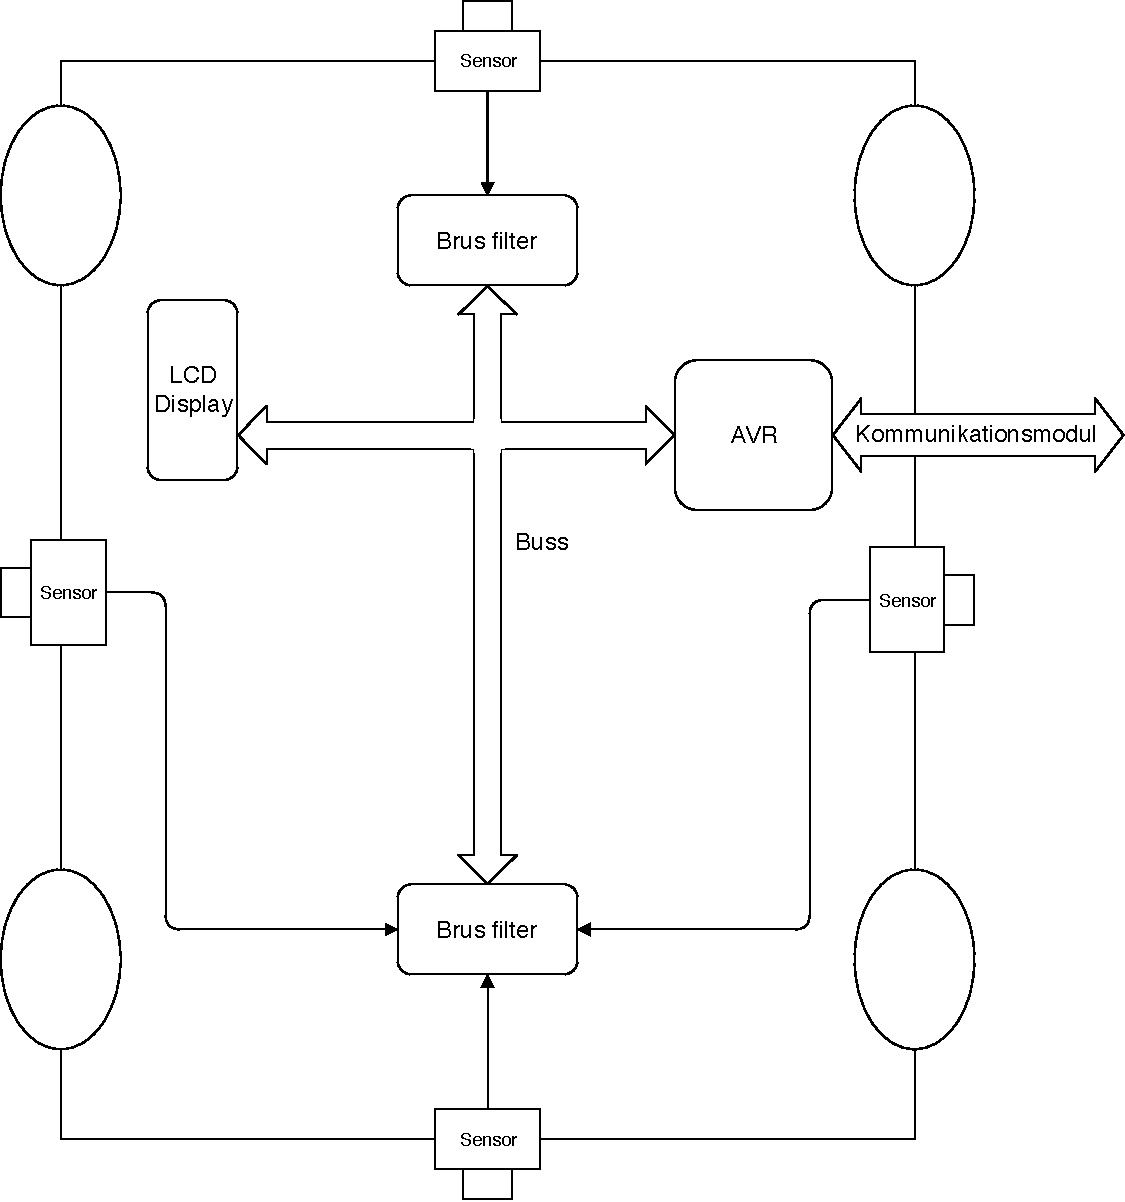
\includegraphics[width=0.6\linewidth]{systemskiss/figures/sensormodul.pdf}
    \caption{Övergripande bild över sensormodulen}
    \label{fig:sensorskiss}
\end{figure}
\noindent
Sensorerna ska vara kopplade till olika brusfilter som ska filtrera bort
störningar av sensorvärdena. Den bakre sensor är tänkt att vara en
IR-avståndsmätare. Bilen kommer använda denna sensor till att upptäcka när den
har kört förbi hinder. Avståndsmätare där framme ska kunna mäta avstånd till
hinder. Det kommer vara antingen en ultraljudssenosr eller en IR-sensor som
åtminstone kan som minst mäta 5 cm och iaf 30 cm framåt eller längre.
Sensorvärden kommer skickas via en databuss till modulens
processor. En LCD-skärm ska kopplas till mikrokontrollern eller direkt till
bussen. På LCD-skärmen ska sensorvärden visas för att förenkla felsökning av modulen. Modulen ska ha en direkt koppling till kommunikationsmodulen via en databuss. Figur \ref{fig:sensorskiss} visar en grov bild över hur modulen ska se ut.


\end{document}

